\documentclass[11pt]{article}
\usepackage{amsmath, amssymb}
\usepackage{geometry}
\geometry{margin=1in}
\usepackage{fancyhdr}
\usepackage{lastpage}
\usepackage{parskip} % Better paragraph spacing
\usepackage{titlesec} % Better section formatting
\usepackage{graphicx}
\usepackage{float}
\usepackage[most]{tcolorbox}
\usepackage{lmodern}
\usepackage{caption}

% Define commands for reusable content
\newcommand{\coursename}{COM-407 Advanced Networks}
\newcommand{\lecturenum}{02}
\newcommand{\lecturedate}{\today}

% Configure section spacing
\titlespacing*{\section}{0pt}{2ex plus 1ex minus .2ex}{1.5ex plus .2ex}
% Header / Footer
\pagestyle{fancy}
\fancyhf{}
\fancyhead[L]{\coursename}
\fancyhead[R]{Lecture \lecturenum}
\fancyfoot[L]{EPFL - Computer Science}
\fancyfoot[C]{Author: Jonathan Dutoit}
\fancyfoot[R]{Page \thepage\ of \pageref{LastPage}}

\begin{document}

\begin{center}
  {\large EPFL - Computer Science} \\[0.5em]
  {\Large \textbf{\coursename}} \\[0.5em]
  {\large Lecture \lecturenum\ --- \lecturedate} \\[0.5em]
  {\large Author: Jonathan Dutoit} \\
  {\large Professor: Pavlos Nikolopoulos}
\end{center}

\vspace{2cm}

\begin{center}
  {\LARGE \textbf{Network Layer IPv4 and IPv6}}
\end{center}

\vspace{1cm}

\section*{Lecture Contents - Internet Protocol (IP)}

\begin{enumerate}
	\item The 2 main rules of IP Unicast
	\item IPv4 addresses
	\item IPv6 addresses
	\item Nats
	\item Host configuration
	\item Hop Limit and TTL
	\item ARP (connection with MAC layer)
\end{enumerate}

\section*{IP Rule #1: Forward packets according to dest IP address}

\textcolor{red}{Why?}

Goal of IP = interconnect all systems in the world using IP addresses

$\Rightarrow$ Each IP address should \textcolor{blue}{uniquely} identify a system

\textcolor{red}{What?}

1. Assign structured addresses:
\begin{itemize}
	\item every network interface has an IP address with \textcolor{blue}{prefix} + \textcolor{red}{suffix}: e.g. \textcolor{blue}{128.178.71.}\textcolor{red}{202}
	\item interfaces within a \textcolor{blue}{subnet} have the \textcolor{blue}{same prefix} $\Rightarrow$ \textcolor{blue}{same subnet mask}
	\item but \textcolor{red}{different} suffix (a.k.a. host part)
\end{itemize}

2. Forward packets according to \textbf{longest prefix match} principle:
\begin{itemize}
	\item every packet contains the destination IP address in its header
	\item every system (i.e. \textbf{host} = end-system or \textbf{router} = intermediate system)
	\begin{itemize}
		\item has a \textbf{forwarding table} (=routing table) and
	\item forwards each packet based on the \textbf{closest} table entry to the destination IP address
	\end{itemize}
\end{itemize}

\section*{Longest prefix match (= \textcolor{red}{closest} matching table entry)}

% Quick centered image
\begin{figure}[H]
    \centering
    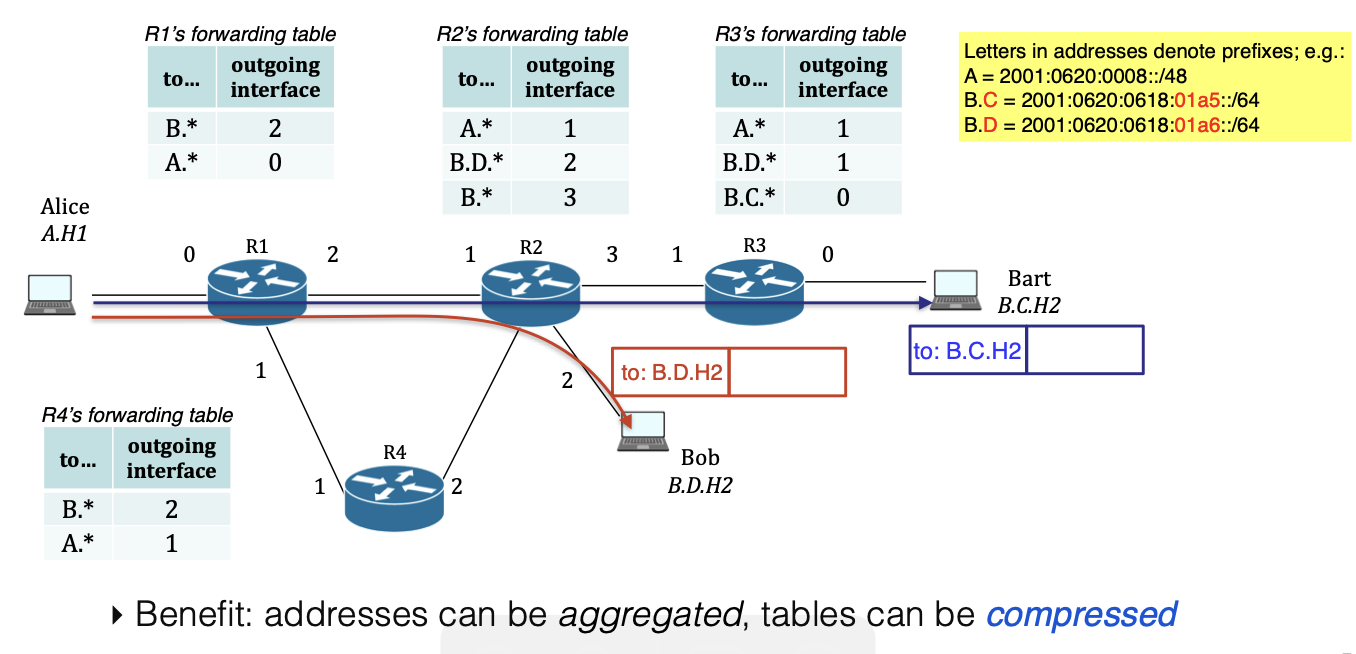
\includegraphics[width=1\textwidth]{prefix-match}
    \label{fig:LABEL}
\end{figure}

\section*{IP Rule #2: Only routers interconnect different LANs/subnets}

$\Rightarrow$ \textcolor{blue}{Between} LANs/subnets, use \textcolor{blue}{routers}

$\Rightarrow$  \textcolor{red}{within} each subnet, do \textcolor{red}{not}. Instead, use data-link-layer forwarding devices within subnet (e.g. switches, wifi base stations, etc.) 

\section*{Question}

\begin{minipage}{0.6\textwidth}
\textbf{Q:} We observe a \textcolor{blue}{packet} from W to P at 1. Which IP destination address do we see?

\vspace{0.5cm}
\begin{enumerate}
        \item The IP address of P
        \item The IP address of an Ethernet interface of the Ethernet switch
	\item There is no destination IP address in the packet since communication is inside the subnet and does not go through a router
\end{enumerate}

\vspace{0.5cm}
\textbf{S:} 1

The IP address is \textcolor{blue}{always present} in the IP Header, even if communication is inside the same LAN

\end{minipage}
\hfill
\begin{minipage}{0.4\textwidth}
\centering
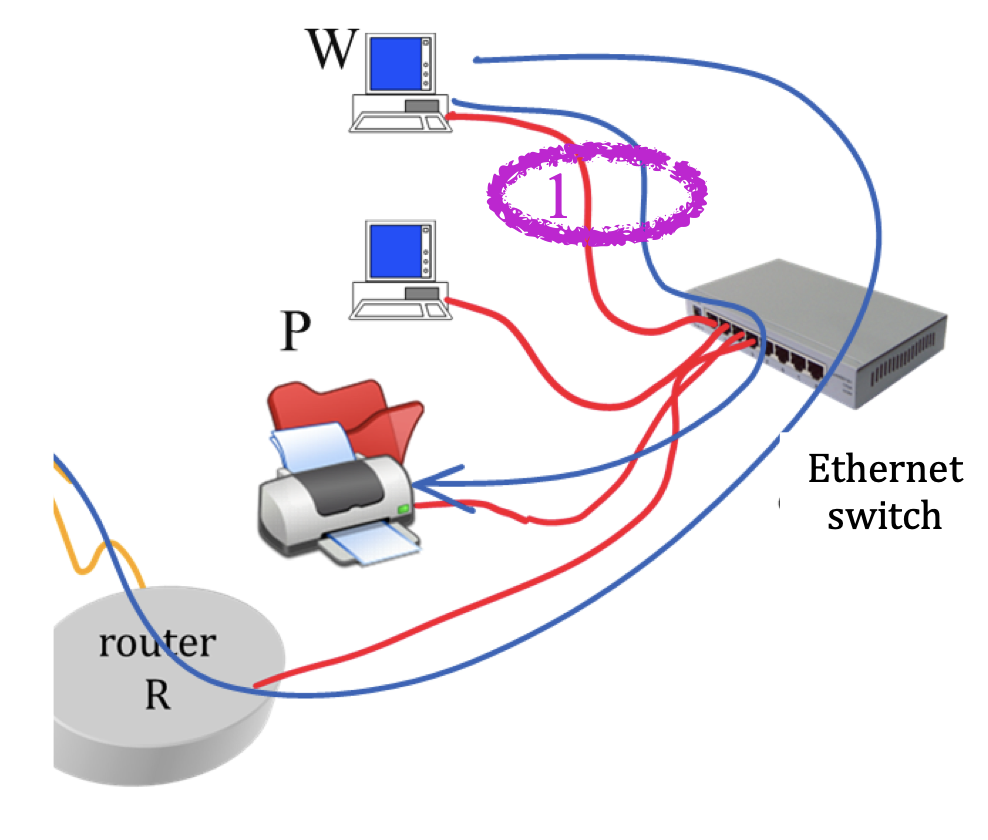
\includegraphics[width=\linewidth]{question-diagram}
\end{minipage}

\newpage

\section*{2. IPv4}

Address format: 32 bits, usually written in dotted decimal notation

\textcolor{red}{binary}: 32 bits
\begin{itemize}
	\item example 1: \textbf{b}1000 0000 1011 1111 1001 0111 0000 0001
	\item example 2: \textbf{b}1000 0001 1100 0000 1100 1000 0000 0010
\end{itemize}

\textcolor{red}{dotted decimal}: 4 integers (one integer = 8bits/binary digits)
\begin{itemize}
	\item example 1: 128.191.151.1
	\item example 2: 129.192.200.2
\end{itemize}

\textcolor{red}{hexadecimal}: 8 hex digits (one hex digit = 4bits/binary digits)
\begin{itemize}
	\item example 1: \textbf{x}80 bf 97 01
	\item example 2: \textbf{x}81 c0 c8 02
\end{itemize}

\section*{Question}

\textbf{Q:} The mask 255.255.254.0 means that the subnet is made of the first...

\begin{enumerate}
	\item 16 bits
	\item 18 bits
	\item 22 bits
	\item 23 bits
	\item 24 bits
\end{enumerate}

\vspace{0.5cm}

\textbf{S:} 4. \textcolor{red}{254} is \textcolor{red}{1111 1110} in binary form $\Rightarrow$ 255.255.254.0 = 1111 1111 1111 1111 \textcolor{red}{1111 1110} 0000 0000 in binary form. So, the mask has 23 contiguous bits equal to 1 starting from the beginning.

\section*{Reserved IPv4 address blocks}

% Quick centered image
\begin{figure}[H]
    \centering
    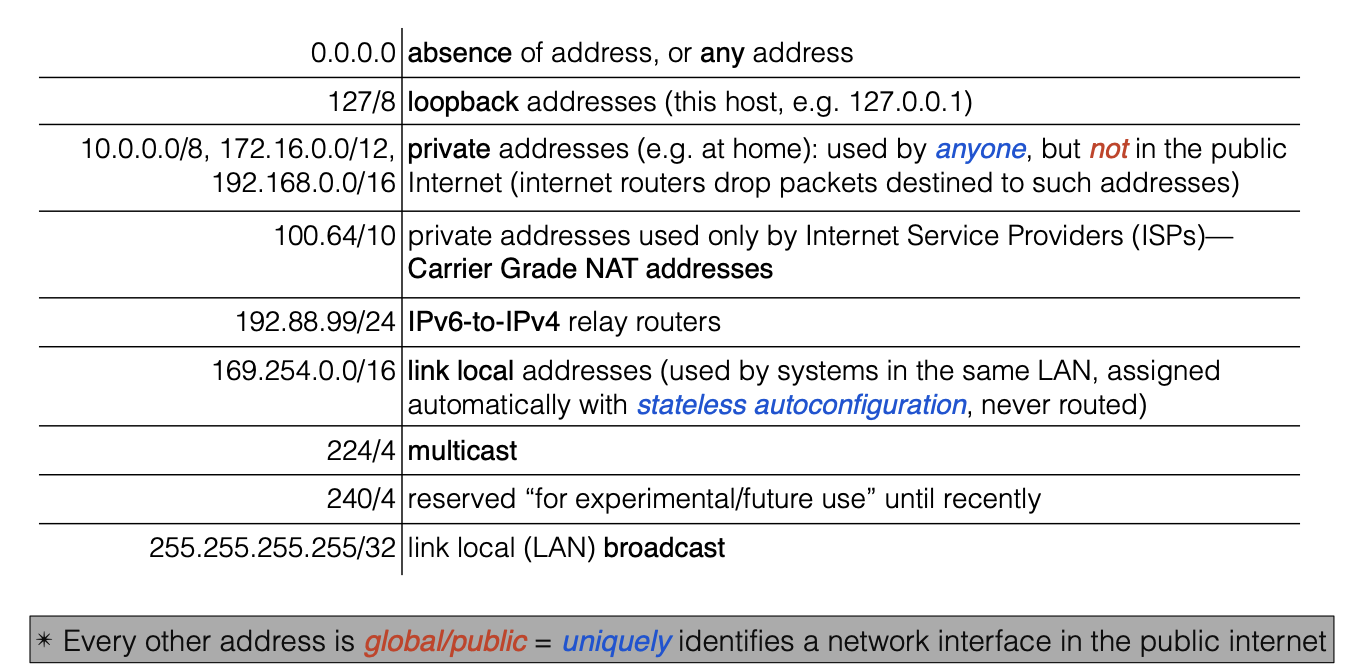
\includegraphics[width=1\textwidth]{ipv4-address-block}
    \label{fig:LABEL}
\end{figure}

\section*{IPv4 Packet Format}

% Quick centered image
\begin{figure}[H]
    \centering
    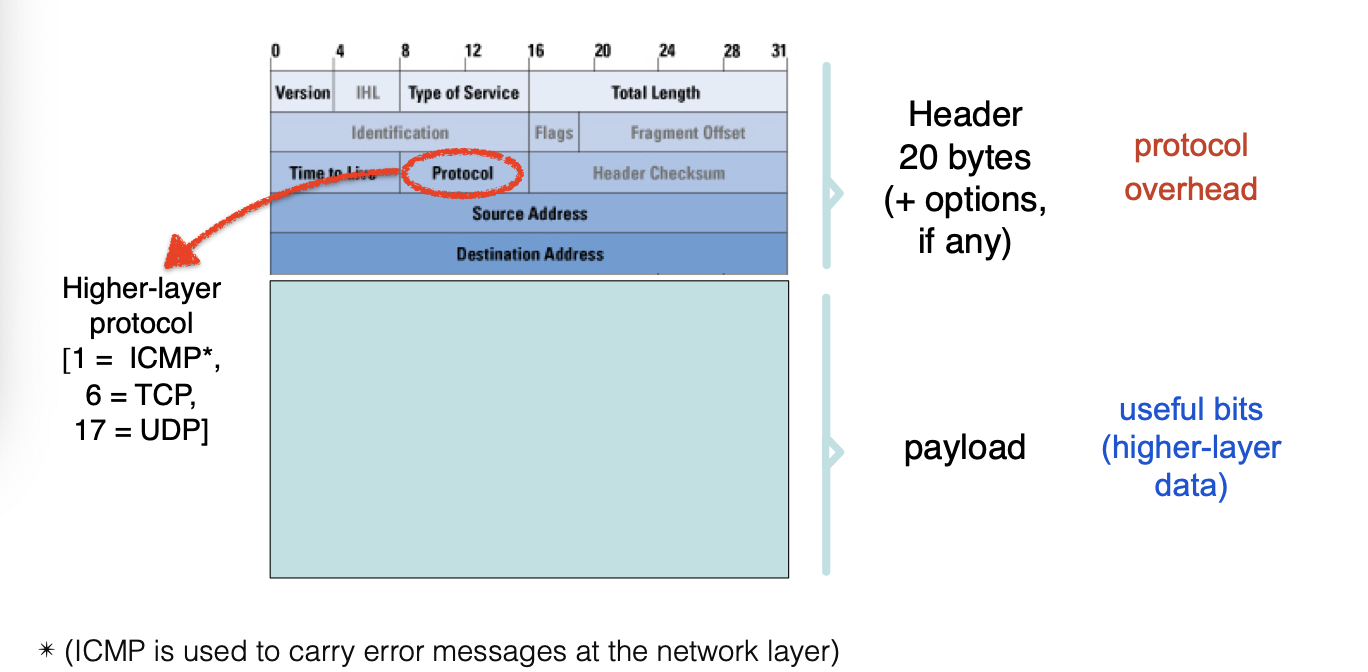
\includegraphics[width=1\textwidth]{ipv4-packet-format}
    \label{fig:LABEL}
\end{figure}

\section*{Forwarding table and longest prefix match: example from EPFL}

% Quick centered image
\begin{figure}[H]
    \centering
    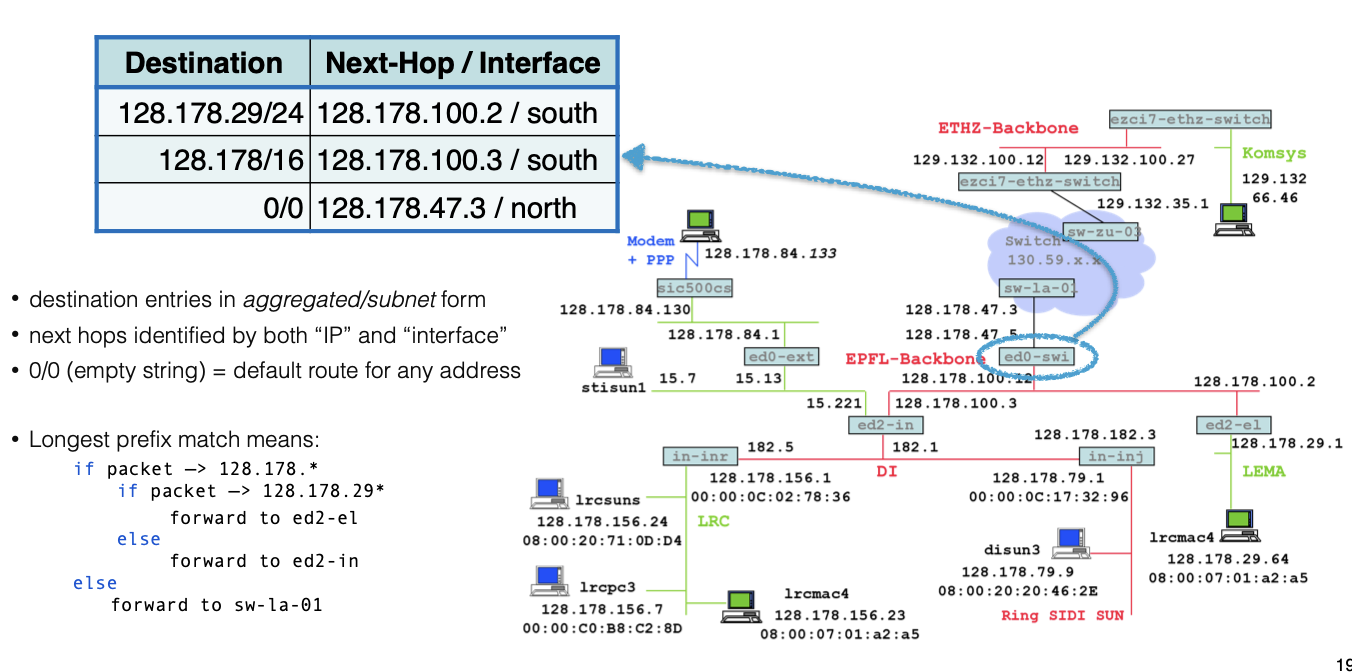
\includegraphics[width=1\textwidth]{longest-prefix-match}
    \label{fig:LABEL}
\end{figure}

\section*{3. IPv6}

\textcolor{red}{Why} a new version? 

IPv4 address space is too small (32 bits $\Rightarrow \approx 4 \cdot 10^{9}$ unique addresses)

\textcolor{red}{What} does IPv6 do?

Redefines packet format with larger addresses of: \textcolor{red}{128 bits} ($\approx 3 \cdot 10^{38}$ unique addresses)

Otherwise, it offers essentially the same services as IPv4

\textcolor{red}{But} IPv6 is \textcolor{blue}{incompatible} with IPv4; routers and host must handle them separately

A can talk to W, B can talk to W, A and B cannot communicate at the network layer

% Quick centered image
\begin{figure}[H]
    \centering
    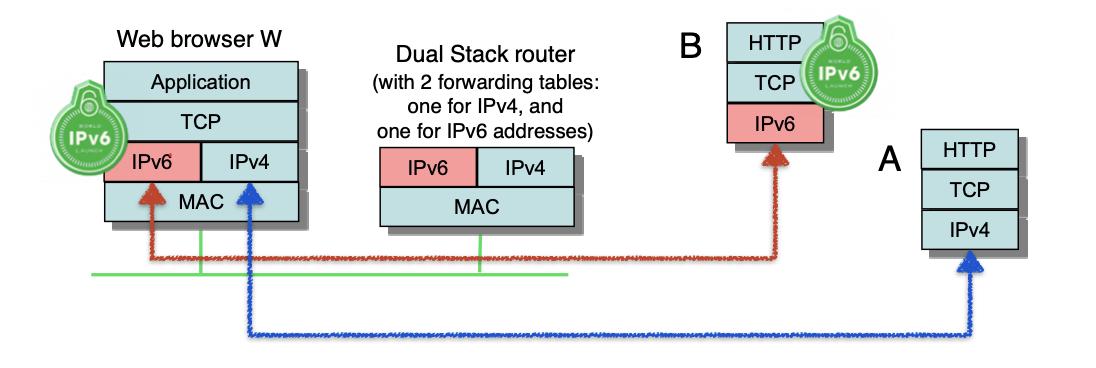
\includegraphics[width=1\textwidth]{ipv6}
    \label{fig:LABEL}
\end{figure}

\section*{IPv6 Address format}
\begin{itemize}
	\item Hex notation with lowercase letters
		\begin{itemize}
			\item 8 hextets separated by ":"
			\item \textbf{hextet} = [0-4] hex digits = 16 bits
		\end{itemize}
	\item Compression Rules
		\begin{itemize}
			\item leading 0s of a hextet can be \textcolor{red}{omitted}
		\item :: replaces any number of 0s in more than one hextet; used \textcolor{blue}{at most once} without ambiguity
		\item 2002:0000:0000:0000:0000:ffff:80b2:0c26 $\Rightarrow$ 2002::ffff:80b2:c26
		\item 2001:0620:0618:01a6:0000:20ff:fe78:30f9 $\Rightarrow$ 2001:620:618:1a6:0:20ff:fe78:30f9
	\end{itemize}
\end{itemize} \section*{Reserved address blocks}

% Quick centered image
\begin{figure}[H]
    \centering
    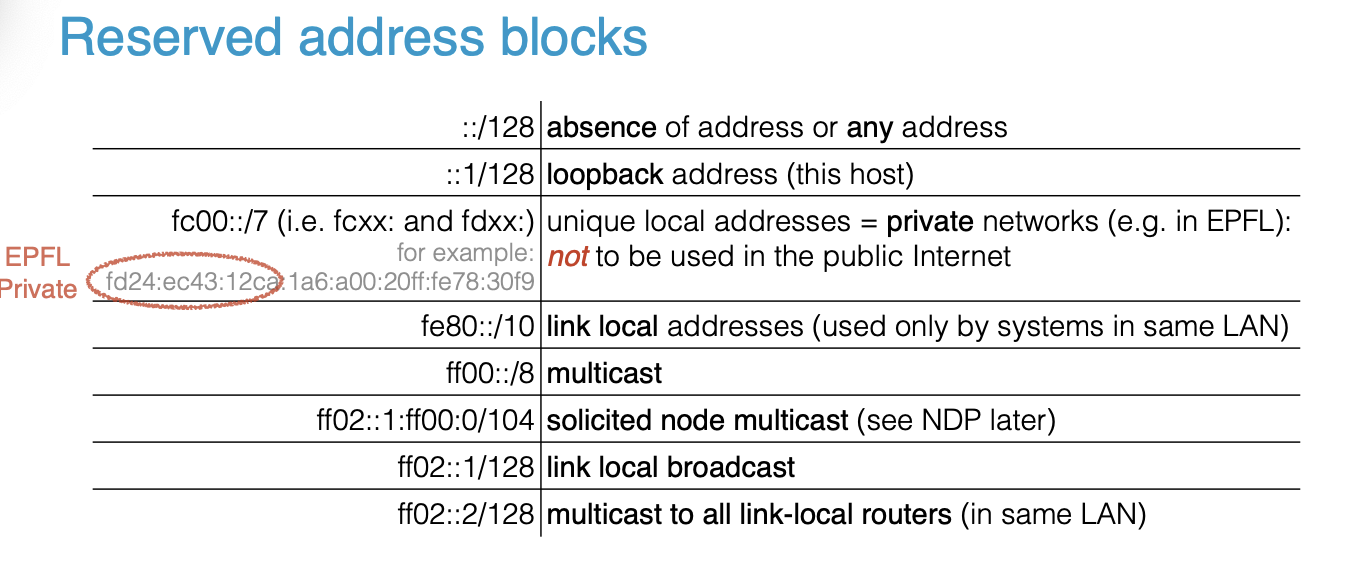
\includegraphics[width=1\textwidth]{ipv6-address-block}
    \label{fig:LABEL}
\end{figure}

\textbf{Note:} IPv6 private prefixes are also allocated, \textcolor{red}{not} reused (in the public internet))

an EPFL public address:
\textcolor{red}{2001:620:618:}1a6:a00:20ff:fe78:30f9

an EPFL private address: 
\textcolor{blue}{fd}\textcolor{red}{24:ec43:12ca}:1a6:a00:20ff:fe78:30f9

\textcolor{blue}{fd} denotes a private address. The red sequence is something specific to EPFL. This is not meant to be reused by someone else. Instead of IPv4 where 192.168.X.X are private addresses for everyone...

\newpage

\section*{A few IPv6 global unicast addresses}

\begin{itemize}
	\item Currently, only the block 2000/3 (i.e. 2xxx and 3xxx) is for global/public unicast addresses.
	% Quick centered image
	\begin{figure}[H]
	    \centering
	    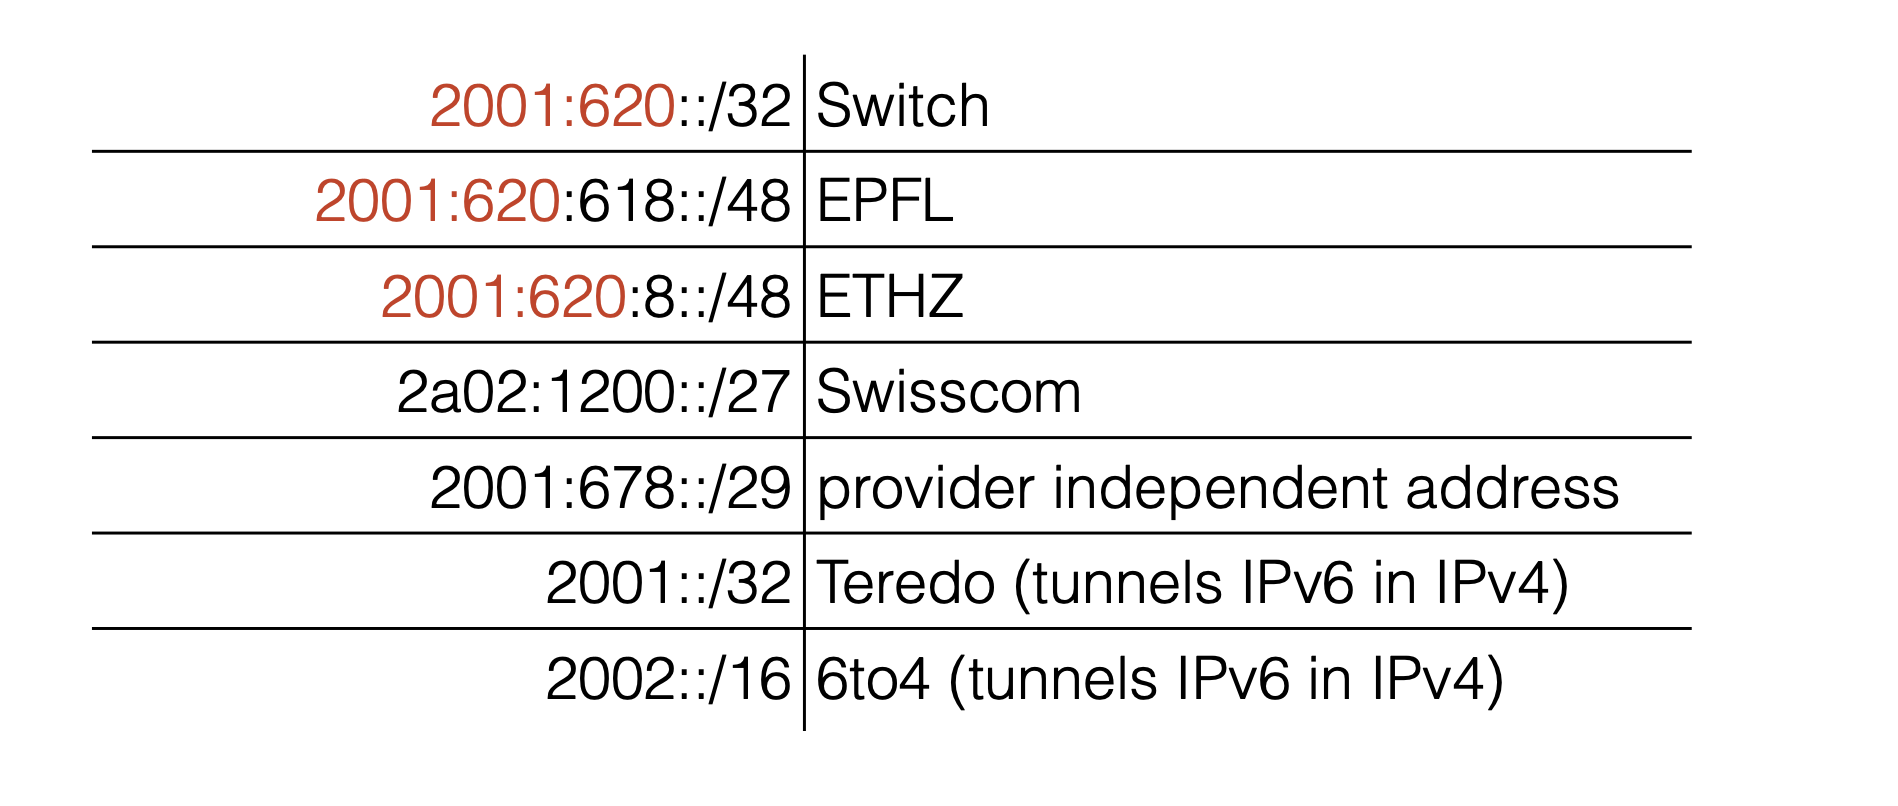
\includegraphics[width=0.7\textwidth]{global-unicast-addresses}
	    \label{fig:LABEL}
	\end{figure}
	\item \textcolor{blue}{Hierarchical allocation}: Networks served by a provider use blocks that are \textcolor{blue}{subnets} of the provider's address block (e.g. check EPFL, ETHZ and SWITCH)
\end{itemize}


\section*{IPv6 Packet Format}

% Quick centered image
\begin{figure}[H]
    \centering
    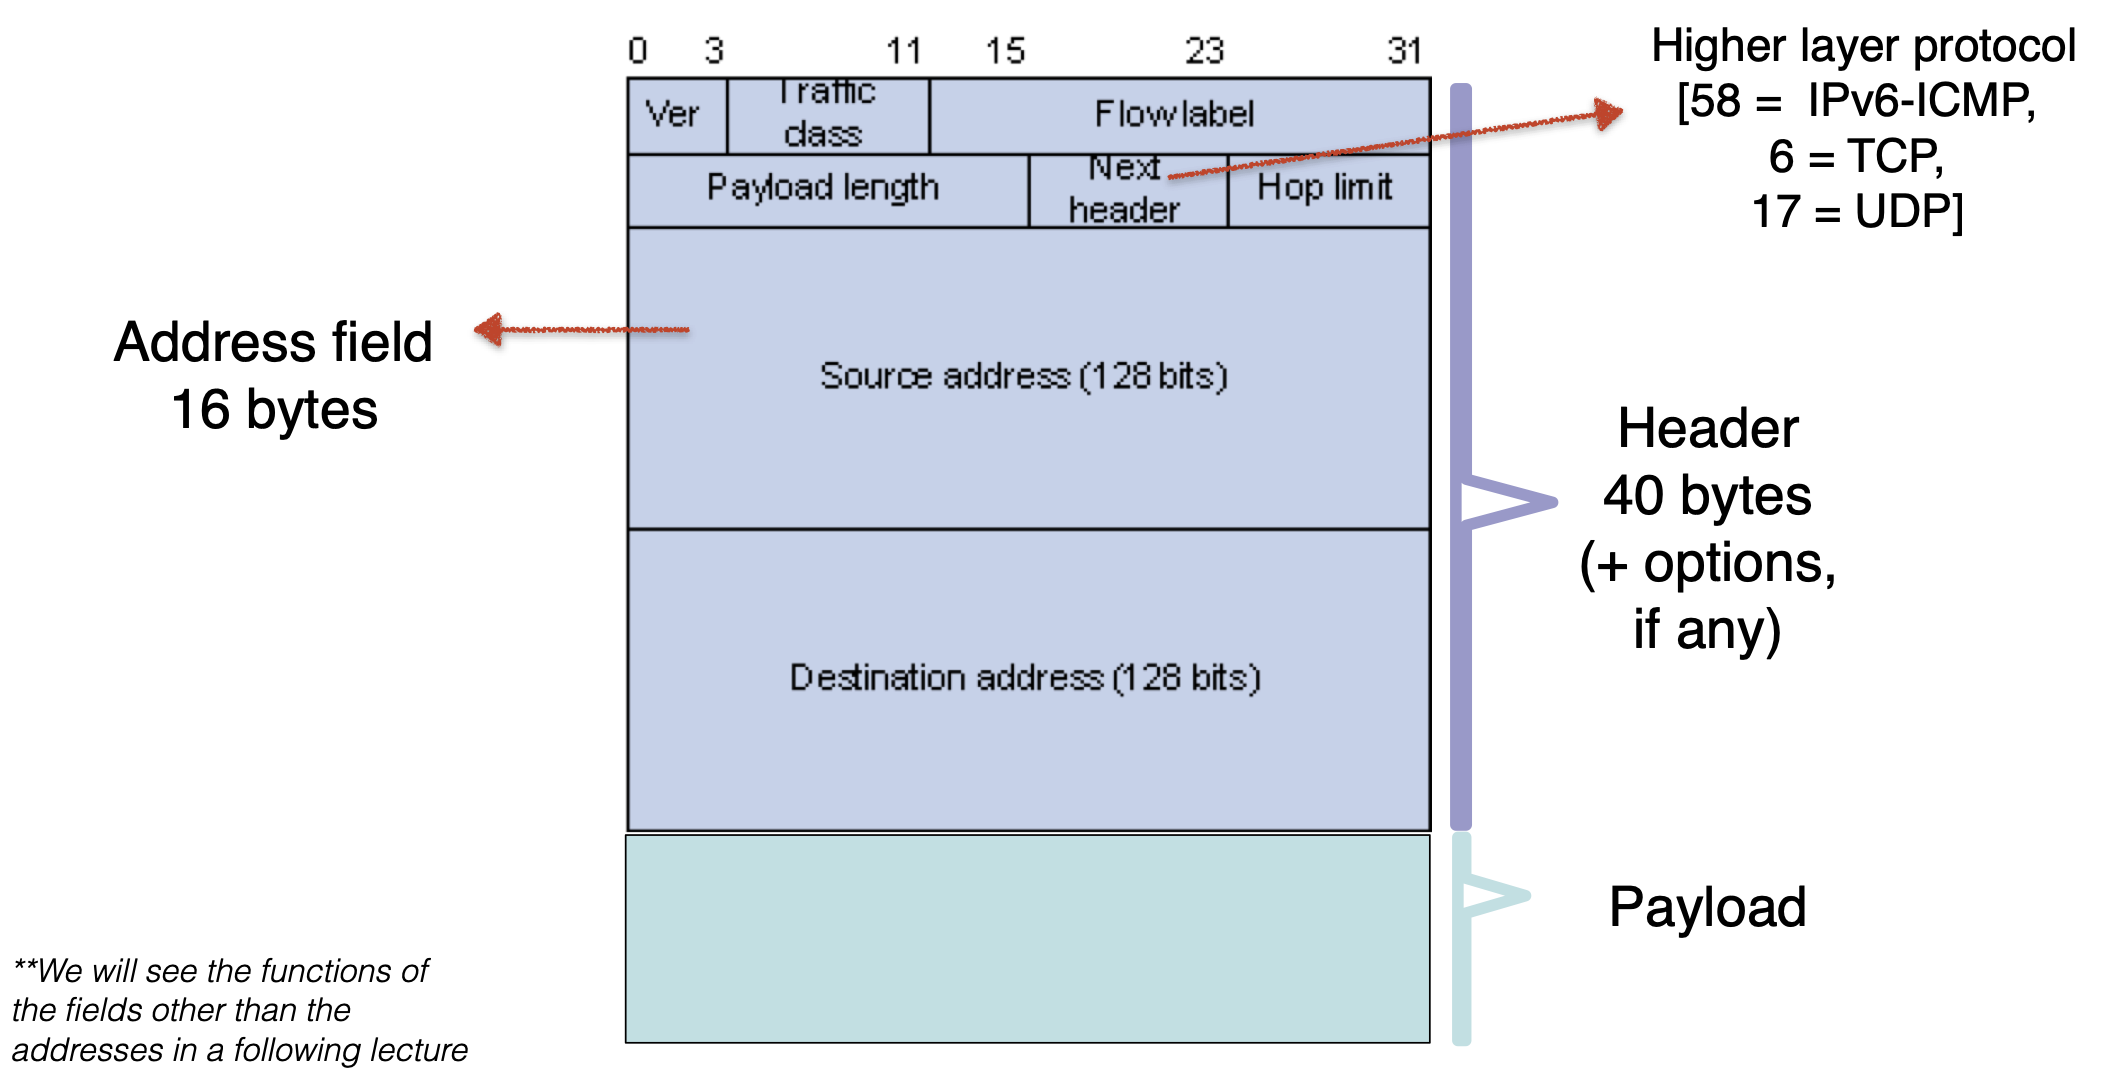
\includegraphics[width=1\textwidth]{ipv6-packet-format}
    \label{fig:LABEL}
\end{figure}

\textbf{Note:} IPv6 is not always a good idea because of big header size (40 bytes) which can make for lower throughputs. For instance, for a IoT setup (multiple physical devices sending data frequently), IPv6 may not be suitable.

% Quick centered image
\begin{figure}[H]
    \centering
    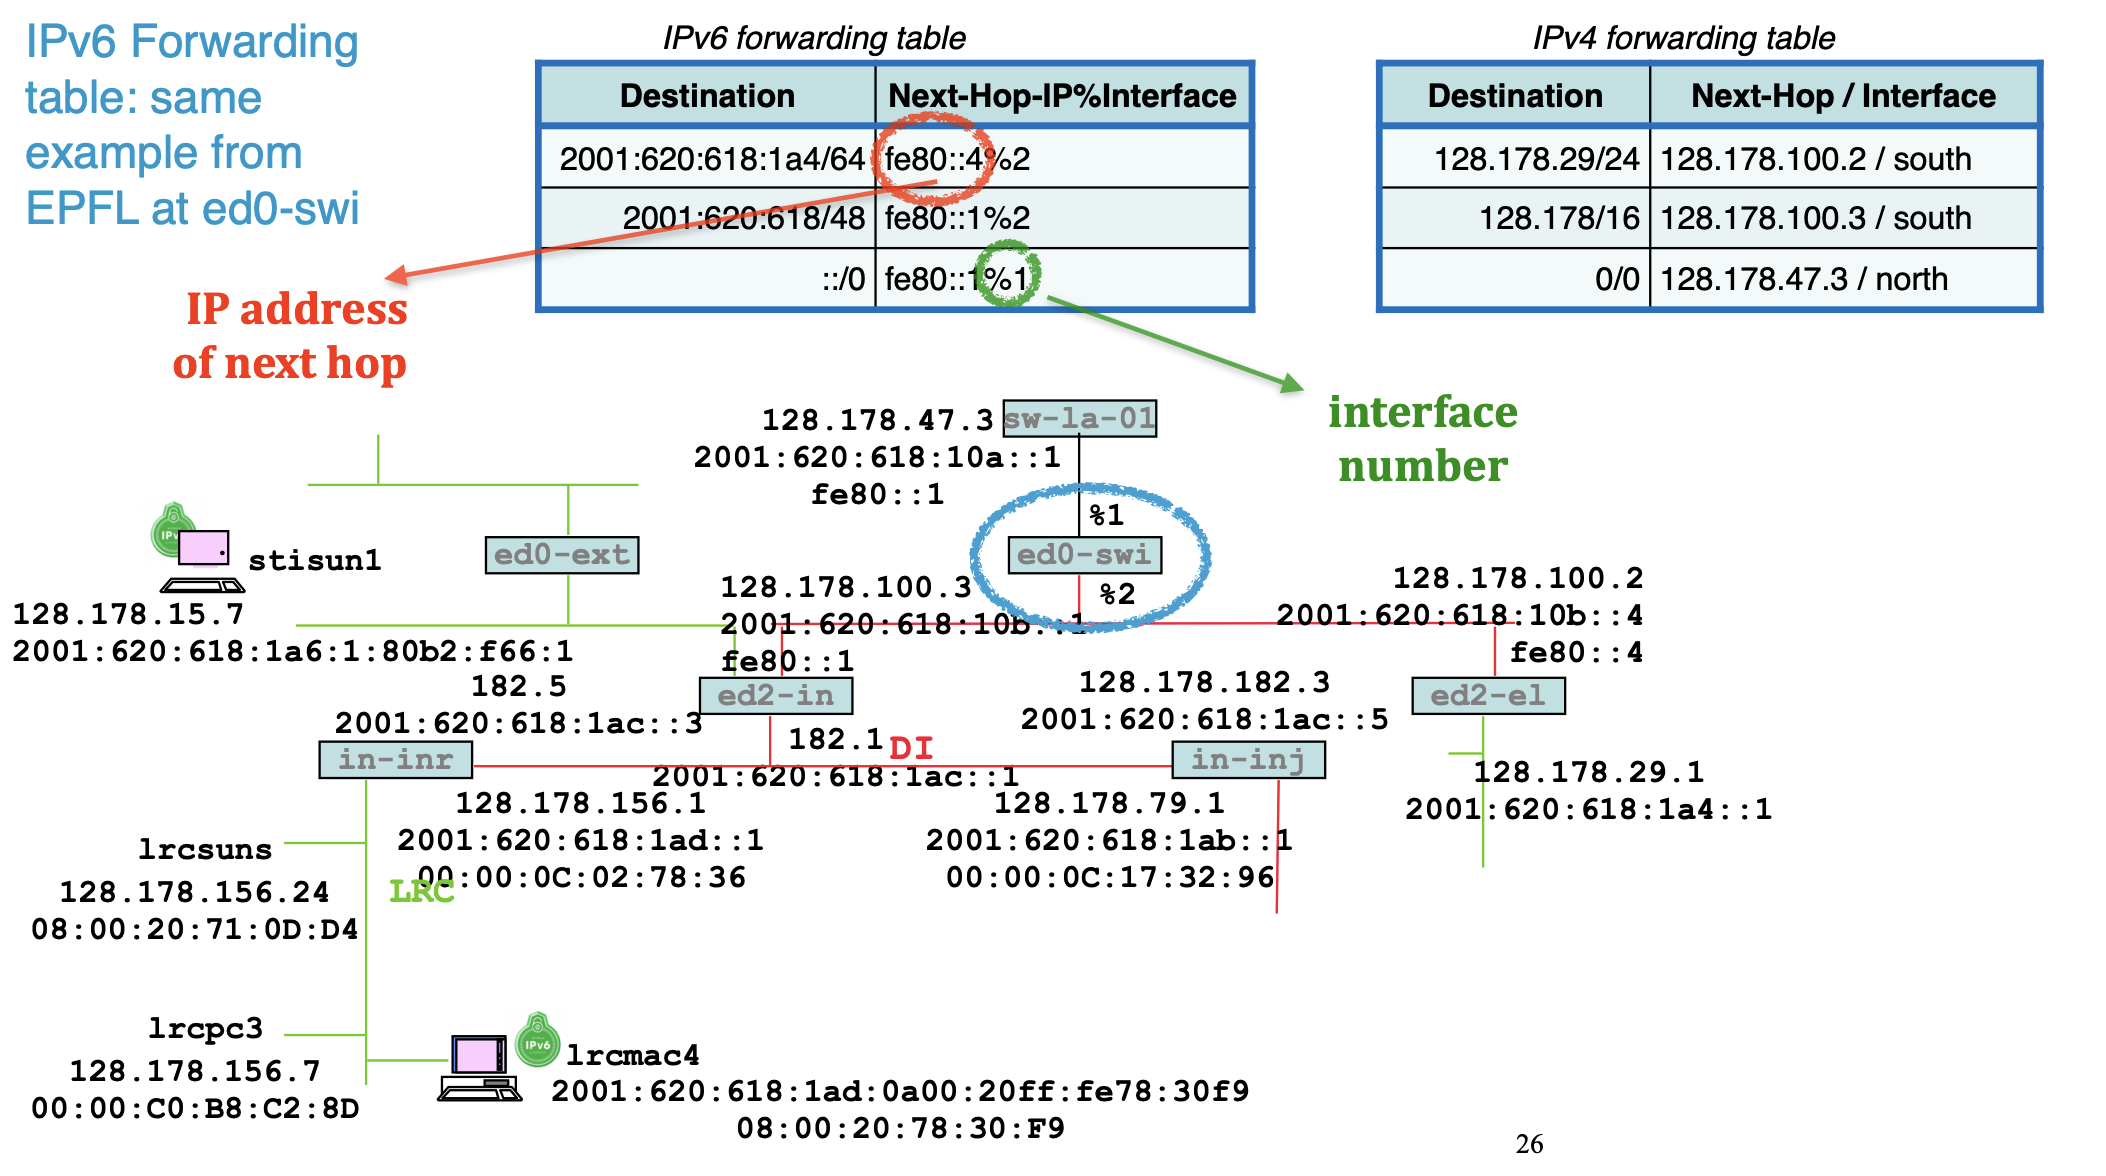
\includegraphics[width=1\textwidth]{ipv6-forwarding-table}
    \label{fig:LABEL}
\end{figure}

\section*{Multiple addresses per interface are the rule with IPv6}

\begin{minipage}{0.6\textwidth}
A host interface typically has \\
\begin{itemize}
	\item one or several \textcolor{red}{link local} addresses
	\item plus one or several global \textcolor{red}{unicast} addresses (secure (GCA) address, temporary addresses) \\
\end{itemize}


The \textcolor{blue}{preference selection algorithm}, configured by OS, says which address should be used as source address - see RFC 3484 \\

In contrast, in IPv4:
there is usually only one IP address per interface
\end{minipage}
\hfill
\begin{minipage}{0.4\textwidth}
\centering
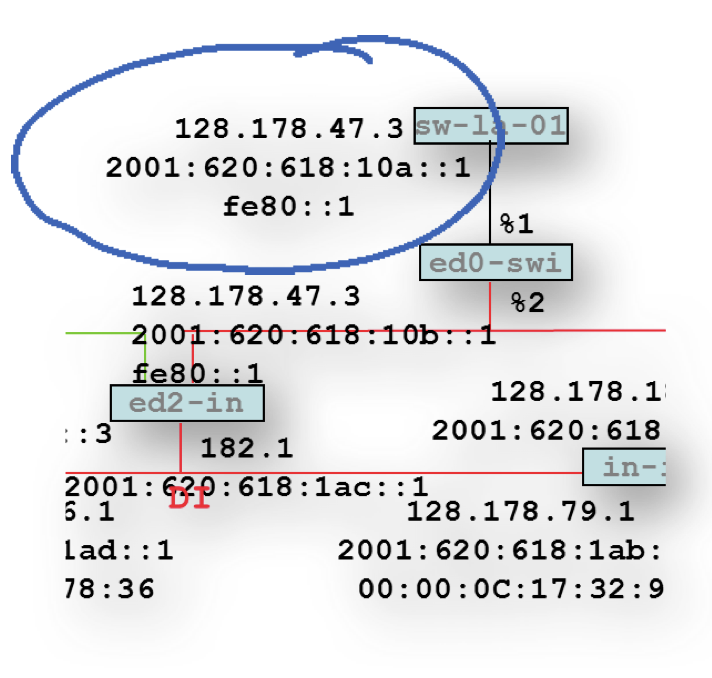
\includegraphics[width=\linewidth]{ipv6-mult-addresses}
\end{minipage}

The \textcolor{blue}{zone index} identifies an interface inside one machine that has several interfaces (e.g. a router)
\begin{itemize}
	\item typically visible in Windows machines
	\item never inside an IP packet
\end{itemize}

E.g. fe80::1\textcolor{blue}{\%2} means: the destination IPv6 address fe80::1 on interface \%2

\section*{4. NAT (Network Address Translation) box}

% Quick centered image
\begin{figure}[H]
    \centering
    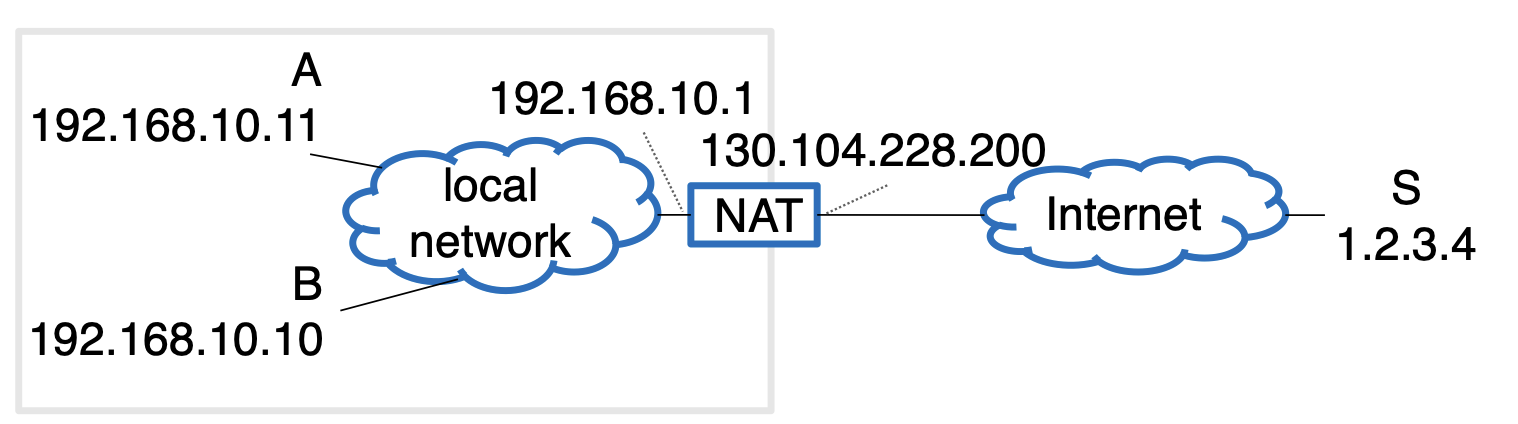
\includegraphics[width=0.7\textwidth]{nat-diagram}
    \label{fig:LABEL}
\end{figure}

\begin{minipage}{0.7\textwidth}
\begin{itemize}
	\item \textcolor{red}{Why} invented? To allow $n > 1$ devices to  \textcolor{blue}{share} a \textcolor{blue}{single} public IP address; e.g.:
	\begin{itemize}
		\item Internet service provider gives you a \textcolor{red}{single} IPv4 address, but you have \textcolor{red}{n devices} at home and need more addresses.
		\item A virtualization platform offers \textcolor{red}{n guest VMs} in one host and allows them to communicate with outside, using \textcolor{red}{the single} IP address of the physical machine \\
	\end{itemize}
	
	\item \textcolor{red}{What} does it do?
	\begin{itemize}
		\item NAT translates (= masquerades) an \textcolor{blue}{internal IP} address and \textcolor{blue}{internal port} number into \textcolor{blue}{NAT IP} address and \textcolor{blue}{NAT port}
		\item Internal addresses are typically \textbf{private}, ports are either UDP or TCP
		\item From outside, one sees only the (\textbf{public}) NAT IP address and a NAT port \\
	\end{itemize}
		
	\item NAT is a \textcolor{blue}{network-layer} middle box, but \textcolor{red}{violates}
	\begin{itemize}
		\item layering $\Rightarrow$ manipulates 2 layers to work (IP and port)
		\item IP rule that public addresses should identify host uniquely \\
	\end{itemize}
\end{itemize}

\end{minipage}
\hfill
\begin{minipage}{0.3\textwidth}
\centering
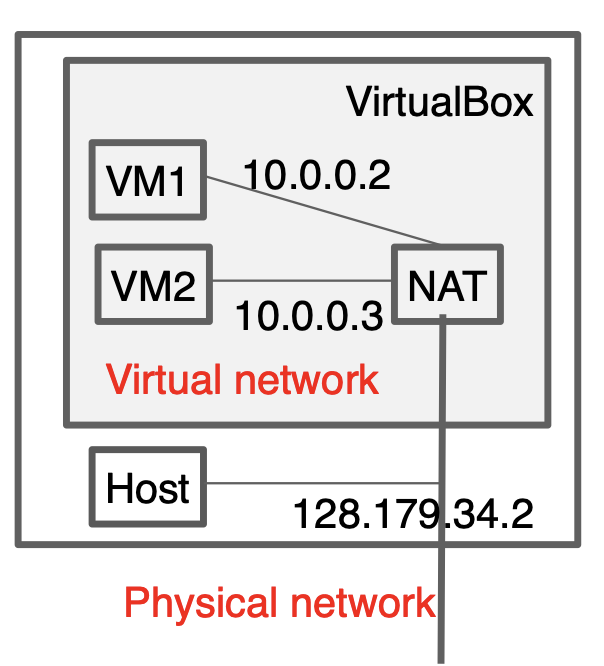
\includegraphics[width=\linewidth]{virtual-box}
\end{minipage}
\textbf{Note:} Also used in IPv6, but very often used for IPv4. Designed for a temporal solution because of missing public addresses from IPv4

\end{document}

